% Implementation chart of the statistical / GAM engine, keyed by the functions
% and objects actually called, with the owning R file on every node.
% Redrawn 2026-09-23 against the call graph from R's own parser
% (callgraph_parse.R -> callgraph/definitions.csv, edges.csv);
% `python docs/figs/callgraph_check.py` checks that every top-level function
% reachable from the engine's entry scripts is named on this chart or
% allow-listed with a reason. Boosters, severity comparators and attribution
% are out of scope here and have their own reachability tables.
%
% Box format: number and purpose (bold), the function(s) it stands for
% (monospace), the functions called inside it (small grey), the owning file.
% Grey dashed notes carry the few facts a reader needs that a name cannot say.
%
% Build:  pdflatex pipeline_implementation.tex   (from this directory)
\documentclass[10pt]{article}
\usepackage[paperwidth=44cm,paperheight=88cm,margin=8mm]{geometry}
\usepackage[T1]{fontenc}
\usepackage{lmodern}
\usepackage{amsmath}
\usepackage{tikz}
\usetikzlibrary{arrows.meta,fit,backgrounds,calc,positioning}
\pagestyle{empty}
\begin{document}
\centering
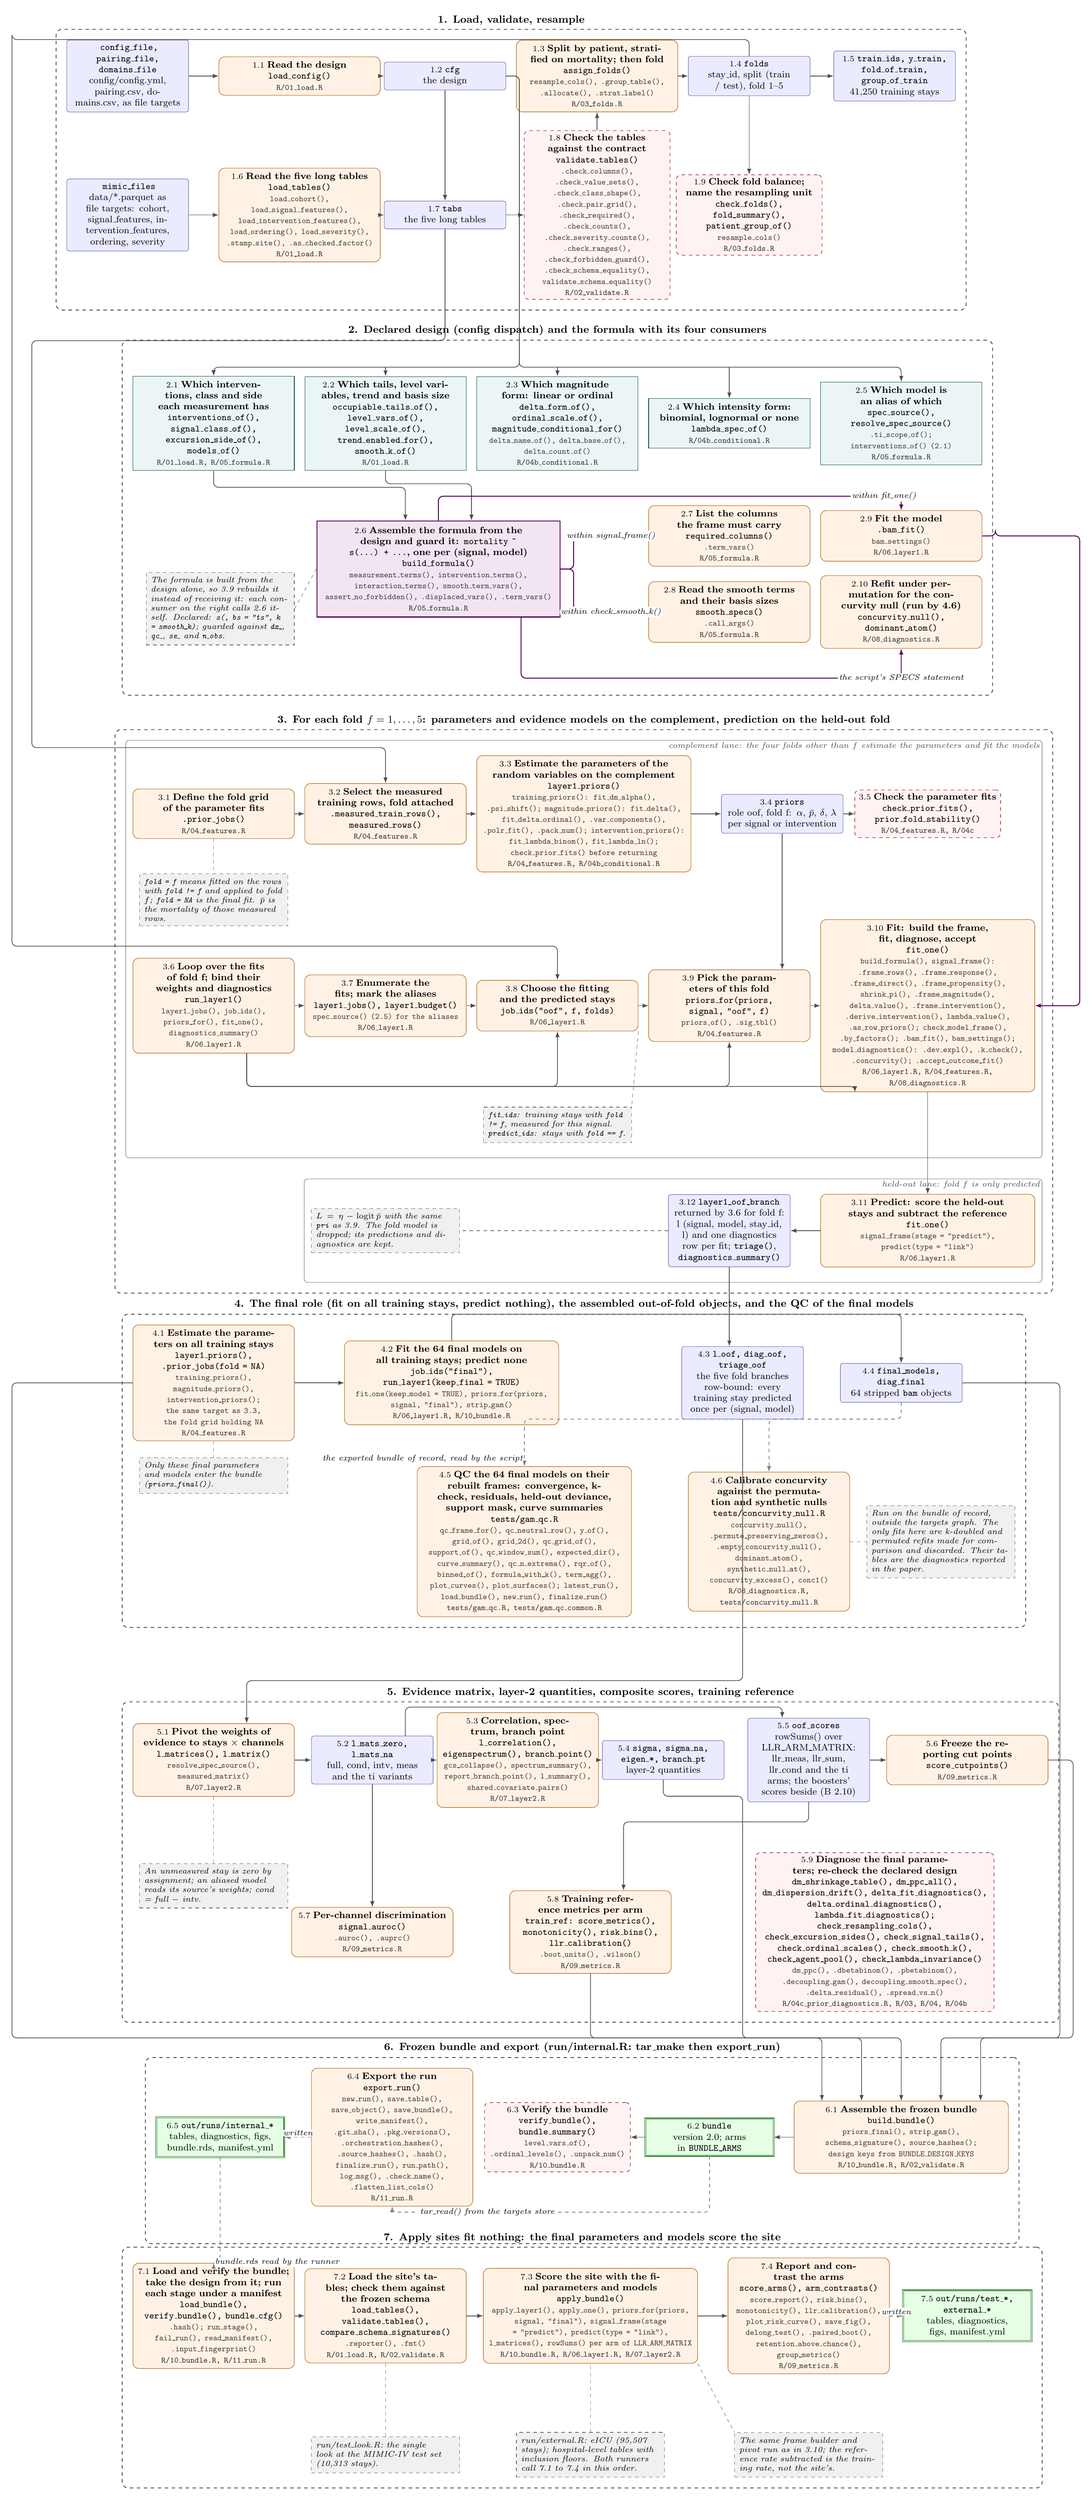
\begin{tikzpicture}[
  font=\footnotesize, x=1cm, y=1cm,
  fn/.style={draw=orange!70!black, fill=orange!10, rounded corners=5pt, align=center, inner sep=4pt, text width=4.6cm},
  fnw/.style={fn, text width=6.2cm},
  obj/.style={draw=blue!50!black!60, fill=blue!8, rounded corners=2pt, align=center, inner sep=4pt, text width=3.4cm},
  chk/.style={draw=red!60!black, fill=red!5, dashed, rounded corners=4pt, align=center, inner sep=3pt, text width=4.2cm},
  dcl/.style={draw=teal!60!black, fill=teal!8, align=center, inner sep=4pt, text width=4.6cm},
  hub/.style={draw=violet!70!black, fill=violet!10, thick, align=center, inner sep=5pt, text width=4.2cm},
  outp/.style={draw=green!40!black, fill=green!10, double, align=center, inner sep=4pt, text width=3.6cm},
  note/.style={draw=black!60, dashed, fill=black!6, align=left, inner sep=4pt, text width=4.2cm, font=\scriptsize\itshape},
  e/.style={-{Latex[length=5pt]}, line width=0.6pt, draw=black!70, rounded corners=4pt},
  ef/.style={e, draw=violet!70!black, thick},
  ex/.style={e, dashed, draw=black!50},
  al/.style={font=\scriptsize\itshape, fill=white, inner sep=1pt},
  en/.style={draw=black!55, dashed, line width=0.4pt},
  grp/.style={draw=black!70, dashed, line width=0.7pt, inner sep=9pt, rounded corners=5pt},
  lane/.style={draw=black!55, inner xsep=6pt, inner ysep=13pt, rounded corners=3pt},
  lab/.style={font=\small\bfseries, anchor=south},
  lanelab/.style={font=\scriptsize\itshape, anchor=north east, text=black!70, inner sep=2pt}]

% number, purpose, function(s), inner calls, file
\newcommand{\B}[5]{{\scriptsize #1}\;\textbf{#2}\\\texttt{\textbf{#3}}\\{\scriptsize\ttfamily\color{black!75}#4}\\{\scriptsize\ttfamily\color{black!80}#5}}
% number, purpose, function(s), file (no inner calls)
\newcommand{\Bs}[4]{{\scriptsize #1}\;\textbf{#2}\\\texttt{\textbf{#3}}\\{\scriptsize\ttfamily\color{black!80}#4}}
% number, object, contents
\newcommand{\Obj}[3]{{\scriptsize #1}\;\texttt{\textbf{#2}}\\#3}

% =====================================================================
% STAGE 1
% =====================================================================
\node[obj] (cfgfiles) at (0,0) {\Obj{}{config\_file, pairing\_file, domains\_file}{config/config.yml, pairing.csv, domains.csv, as file targets}};
\node[fn]  (loadcfg) at (5.2,0) {\Bs{1.1}{Read the design}{load\_config()}{R/01\_load.R}};
\node[obj] (cfg) at (9.6,0) {\Obj{1.2}{cfg}{the design}};
\node[fn]  (folds) at (14.2,0) {\B{1.3}{Split by patient, stratified on mortality; then fold}{assign\_folds()}{resample\_cols(), .group\_table(), .allocate(), .strat\_label()}{R/03\_folds.R}};
\node[obj] (foldsobj) at (18.8,0) {\Obj{1.4}{folds}{stay\_id, split (train / test), fold 1--5}};
\node[obj] (trainobj) at (23.2,0) {\Obj{1.5}{train\_ids, y\_train, fold\_of\_train, group\_of\_train}{41,250 training stays}};

\node[obj] (parq) at (0,-4.2) {\Obj{}{mimic\_files}{data/*.parquet as file targets: cohort, signal\_features, intervention\_features, ordering, severity}};
\node[fn]  (loadt) at (5.2,-4.2) {\B{1.6}{Read the five long tables}{load\_tables()}{load\_cohort(), load\_signal\_features(), load\_intervention\_features(), load\_ordering(), load\_severity(), .stamp\_site(), .as\_checked\_factor()}{R/01\_load.R}};
\node[obj] (tabs) at (9.6,-4.2) {\Obj{1.7}{tabs}{the five long tables}};
\node[chk] (valid) at (14.2,-4.2) {\B{1.8}{Check the tables against the contract}{validate\_tables()}{.check\_columns(), .check\_value\_sets(), .check\_class\_shape(), .check\_pair\_grid(), .check\_required(), .check\_counts(), .check\_severity\_counts(), .check\_ranges(), .check\_forbidden\_guard(), .check\_schema\_equality(), validate\_schema\_equality()}{R/02\_validate.R}};
\node[chk] (foldchk) at (18.8,-4.2) {\B{1.9}{Check fold balance; name the resampling unit}{check\_folds(), fold\_summary(), patient\_group\_of()}{resample\_cols()}{R/03\_folds.R}};

\draw[e] (cfgfiles) -- (loadcfg); \draw[e] (loadcfg) -- (cfg);
\draw[e] (parq) -- (loadt); \draw[e] (loadt) -- (tabs); \draw[e] (tabs) -- (valid);
\draw[e] (cfg.south) -- (tabs.north);
\draw[e] (valid.north) -- (folds.south);
\draw[e] (folds) -- (foldsobj); \draw[e] (foldsobj) -- (foldchk); \draw[e] (foldsobj) -- (trainobj);

\begin{scope}[on background layer]
\node[grp, fit=(cfgfiles)(loadcfg)(cfg)(parq)(loadt)(tabs)(valid)(folds)(foldsobj)(foldchk)(trainobj),
  label={[lab]north:1. Load, validate, resample}] (b1) {};
\end{scope}

\begin{scope}[yshift=-0.9cm]
% =====================================================================
% STAGE 2
% =====================================================================
\node[dcl] (dpair) at (2.6,-9.6) {\Bs{2.1}{Which interventions, class and side each measurement has}{interventions\_of(), signal\_class\_of(), excursion\_side\_of(), models\_of()}{R/01\_load.R, R/05\_formula.R}};
\node[dcl] (dmeas) at (7.8,-9.6) {\Bs{2.2}{Which tails, level variables, trend and basis size}{occupiable\_tails\_of(), level\_vars\_of(), level\_scale\_of(), trend\_enabled\_for(), smooth\_k\_of()}{R/01\_load.R}};
\node[dcl] (ddelta) at (13.0,-9.6) {\B{2.3}{Which magnitude form: linear or ordinal}{delta\_form\_of(), ordinal\_scale\_of(), magnitude\_conditional\_for()}{delta\_name\_of(), delta\_base\_of(), delta\_count\_of()}{R/04b\_conditional.R}};
\node[dcl] (dlambda) at (18.2,-9.6) {\Bs{2.4}{Which intensity form: binomial, lognormal or none}{lambda\_spec\_of()}{R/04b\_conditional.R}};
\node[dcl] (dalias) at (23.4,-9.6) {\B{2.5}{Which model is an alias of which}{spec\_source(), resolve\_spec\_source()}{.ti\_scope\_of(); interventions\_of() (2.1)}{R/05\_formula.R}};

\node[hub, text width=7.0cm] (bf) at (9.4,-14) {\B{2.6}{Assemble the formula from the design and guard it: \texttt{mortality \~{} s(\ldots) + \ldots}, one per (signal, model)}{build\_formula()}{measurement\_terms(), intervention\_terms(), interaction\_terms(), smooth\_term\_vars(), assert\_no\_forbidden(), .displaced\_vars(), .term\_vars()}{R/05\_formula.R}};

\node[fn] (fconsume1) at (18.2,-13) {\B{2.7}{List the columns the frame must carry}{required\_columns()}{.term\_vars()}{R/05\_formula.R}};
\node[fn] (fconsume2) at (18.2,-15.3) {\B{2.8}{Read the smooth terms and their basis sizes}{smooth\_specs()}{.call\_args()}{R/05\_formula.R}};
\node[fn] (fconsume3) at (23.4,-13) {\B{2.9}{Fit the model}{.bam\_fit()}{bam\_settings()}{R/06\_layer1.R}};
\node[fn] (fconsume4) at (23.4,-15.3) {\Bs{2.10}{Refit under permutation for the concurvity null (run by 4.6)}{concurvity\_null(), dominant\_atom()}{R/08\_diagnostics.R}};
\node[note] (n1) at (2.8,-15.2) {The formula is built from the design alone, so 3.9 rebuilds it instead of receiving it: each consumer on the right calls 2.6 itself. Declared: \texttt{s(, bs = "ts", k = smooth\_k)}; guarded against \texttt{dx\_}, \texttt{qc\_}, \texttt{se\_} and \texttt{n\_obs}.};

% every dispatcher reads the design object 1.2 (a bus down the lane between 1.7 and 1.8)
\draw[e] (cfg.east) -- ++(0.4,0) |- (2.6,-7.9) -- (dpair.north);
\draw[e] (cfg.east) -- ++(0.4,0) |- (23.4,-7.9) -- (dalias.north);
\draw[e] (7.8,-7.9) -- (dmeas.north); \draw[e] (13.0,-7.9) -- (ddelta.north); \draw[e] (18.2,-7.9) -- (dlambda.north);
\draw[e] (dpair.south) -- ++(0,-0.5) -| ($(bf.north)+(-1.0,0)$);
\draw[e] (dmeas.south) -- ++(0,-0.4) -| ($(bf.north)+(1.0,0)$);
\draw[ef] (bf.east) -- ++(0.4,0) |- (fconsume1.west) node[al, pos=0.75] {within signal\_frame()};
\draw[ef] (bf.east) -- ++(0.4,0) |- (fconsume2.west) node[al, pos=0.75] {within check\_smooth\_k()};
\draw[ef] (bf.north) |- (20.8,-11.8) -| (fconsume3.north) node[al, pos=0.4] {within fit\_one()};
\draw[en] (bf.west) -- (n1.east);
\draw[ef] ($(bf.south)+(2.5,0)$) |- (20.8,-17.3) -| (fconsume4.south) node[al, pos=0.5] {the script's SPECS statement};

\begin{scope}[on background layer]
\node[grp, fit={(dpair)(dmeas)(ddelta)(dlambda)(dalias)(bf)(fconsume1)(fconsume2)(fconsume3)(fconsume4)(n1)(2.6,-7.4)(20.8,-17.5)},
  label={[lab]north:2. Declared design (config dispatch) and the formula with its four consumers}] (b2) {};
\end{scope}

% =====================================================================
% STAGE 3: one fold
% =====================================================================
\node[fn] (pj) at (2.6,-21.4) {\Bs{3.1}{Define the fold grid of the parameter fits}{.prior\_jobs()}{R/04\_features.R}};
\node[fn] (mtr) at (7.8,-21.4) {\Bs{3.2}{Select the measured training rows, fold attached}{.measured\_train\_rows(), measured\_rows()}{R/04\_features.R}};
\node[fnw] (pfit) at (13.8,-21.4) {\B{3.3}{Estimate the parameters of the random variables on the complement}{layer1\_priors()}{training\_priors(): fit\_dm\_alpha(), .psi\_shift(); magnitude\_priors(): fit\_delta(), fit\_delta\_ordinal(), .var\_components(), .polr\_fit(), .pack\_num(); intervention\_priors(): fit\_lambda\_binom(), fit\_lambda\_ln(); check\_prior\_fits() before returning}{R/04\_features.R, R/04b\_conditional.R}};
\node[obj] (prf) at (19.8,-21.4) {\Obj{3.4}{priors}{role oof, fold f: $\alpha$, $\bar p$, $\delta$, $\lambda$ per signal or intervention}};
\node[chk] (prchk) at (24.2,-21.4) {\Bs{3.5}{Check the parameter fits}{check\_prior\_fits(), prior\_fold\_stability()}{R/04\_features.R, R/04c}};
\node[note] (n2) at (2.6,-24) {\texttt{fold = f} means fitted on the rows with \texttt{fold != f} and applied to fold $f$; \texttt{fold = NA} is the final fit. $\bar p$ is the mortality of those measured rows.};

\node[fn] (rl1) at (2.6,-27.2) {\B{3.6}{Loop over the fits of fold f; bind their weights and diagnostics}{run\_layer1()}{layer1\_jobs(), job\_ids(), priors\_for(), fit\_one(), diagnostics\_summary()}{R/06\_layer1.R}};
\node[fn] (jobs) at (7.8,-27.2) {\B{3.7}{Enumerate the fits; mark the aliases}{layer1\_jobs(), layer1\_budget()}{spec\_source() (2.5) for the aliases}{R/06\_layer1.R}};
\node[fn] (jid) at (13.0,-27.2) {\Bs{3.8}{Choose the fitting and the predicted stays}{job\_ids("oof", f, folds)}{R/06\_layer1.R}};
\node[fn] (pfor) at (18.2,-27.2) {\B{3.9}{Pick the parameters of this fold}{priors\_for(priors, signal, "oof", f)}{priors\_of(), .sig\_tbl()}{R/04\_features.R}};
\node[fnw] (fit) at (24.2,-27.2) {\B{3.10}{Fit: build the frame, fit, diagnose, accept}{fit\_one()}{build\_formula(), signal\_frame(): .frame\_rows(), .frame\_response(), .frame\_direct(), .frame\_propensity(), shrink\_pi(), .frame\_magnitude(), delta\_value(), .frame\_intervention(), .derive\_intervention(), lambda\_value(), .as\_row\_priors(); check\_model\_frame(), .by\_factors(); .bam\_fit(), bam\_settings(); model\_diagnostics(): .dev\_expl(), .k\_check(), .concurvity(); .accept\_outcome\_fit()}{R/06\_layer1.R, R/04\_features.R, R/08\_diagnostics.R}};
\node[note] (n3) at (13.0,-30.8) {\texttt{fit\_ids}: training stays with \texttt{fold != f}, measured for this signal. \texttt{predict\_ids}: stays with \texttt{fold == f}.};

\node[fnw] (pred) at (24.2,-34.0) {\B{3.11}{Predict: score the held-out stays and subtract the reference}{fit\_one()}{signal\_frame(stage = "predict"), predict(type = "link")}{R/06\_layer1.R}};
\node[obj] (lf) at (18.2,-34.0) {\Obj{3.12}{layer1\_oof\_branch}{returned by 3.6 for fold f: l (signal, model, stay\_id, l) and one diagnostics row per fit; \texttt{triage()}, \texttt{diagnostics\_summary()}}};

\node[note] (n4) at (7.8,-34.0) {$L = \eta - \operatorname{logit}\bar p$ with the same \texttt{pri} as 3.9. The fold model is dropped; its predictions and diagnostics are kept.};

\draw[e] (pj) -- (mtr); \draw[e] (mtr) -- (pfit); \draw[e] (pfit) -- (prf); \draw[e] (prf) -- (prchk);
\draw[e] (rl1) -- (jobs);
\draw[e] ($(rl1.south)+(1.0,0)$) -- ++(0,-1.0) -| (jid.south);
\draw[e] ($(rl1.south)+(1.0,0)$) -- ++(0,-1.0) -| (pfor.south);
\draw[e] ($(rl1.south)+(1.0,0)$) -- ++(0,-1.0) -| ($(fit.south)+(-2.2,0)$);
\draw[e] (jobs) -- (jid); \draw[e] (jid) -- (pfor); \draw[e] (pfor) -- (fit);
\draw[e] (prf.south) -- (prf.south |- pfor.north);
\draw[e] (fit) -- (pred);
\draw[e] (pred) -- (lf);
\draw[en] (pj.south) -- (n2.north);
\draw[en] (jid.south east) -- (n3.north east);
\draw[en] (lf.west) -- (n4.east);

\begin{scope}[on background layer]
\node[lane, fit=(pj)(mtr)(pfit)(prf)(prchk)(n2)(rl1)(jobs)(jid)(pfor)(fit)(n3), label={[lanelab]north east:complement lane: the four folds other than $f$ estimate the parameters and fit the models}] (lane1) {};
\node[lane, fit=(pred)(lf)(n4), label={[lanelab]north east:held-out lane: fold $f$ is only predicted}] (lane2) {};
\end{scope}
\begin{scope}[on background layer]
\node[grp, fit=(lane1)(lane2),
  label={[lab]north:3. For each fold $f = 1,\dots,5$: parameters and evidence models on the complement, prediction on the held-out fold}] (b3) {};
\end{scope}

\draw[ef] (fconsume3.east) -- ++(0.4,0) |- (28.8,-13) |- (fit.east);
\draw[e] (tabs.south) -- (9.6,-7.1) -- (-2.9,-7.1) -- (-2.9,-19.4) -- (7.8,-19.4) -- (mtr.north);
\draw[e] (foldsobj.north) -- ++(0,0.5) -| (-3.5,2.1) |- (13.0,-25.4) -- (jid.north);

% =====================================================================
% STAGE 4
% =====================================================================
\node[fn] (fpri) at (2.6,-38.6) {\B{4.1}{Estimate the parameters on all training stays}{layer1\_priors(), .prior\_jobs(fold = NA)}{training\_priors(), magnitude\_priors(), intervention\_priors(); the same target as 3.3, the fold grid holding NA}{R/04\_features.R}};
\node[fnw] (ffit) at (9.8,-38.6) {\B{4.2}{Fit the 64 final models on all training stays; predict none}{job\_ids("final"), run\_layer1(keep\_final = TRUE)}{fit\_one(keep\_model = TRUE), priors\_for(priors, signal, "final"), strip\_gam()}{R/06\_layer1.R, R/10\_bundle.R}};
\node[obj] (loof) at (18.6,-38.6) {\Obj{4.3}{l\_oof, diag\_oof, triage\_oof}{the five fold branches row-bound: every training stay predicted once per (signal, model)}};
\node[obj] (fmodels) at (23.4,-38.6) {\Obj{4.4}{final\_models, diag\_final}{64 stripped \texttt{bam} objects}};
\node[note] (n5) at (2.6,-41.4) {Only these final parameters and models enter the bundle (\texttt{priors\_final()}).};

\draw[e] (fpri) -- (ffit);
\draw[e] (ffit.north) -- ++(0,0.8) -| (fmodels.north);
\draw[e] (lf.south) -- (lf.south |- loof.north);
\draw[en] (fpri.south) -- (n5.north);

\node[fnw] (qc) at (12.0,-43.4) {\B{4.5}{QC the 64 final models on their rebuilt frames: convergence, k-check, residuals, held-out deviance, support mask, curve summaries}{tests/gam\_qc.R}{qc\_frame\_for(), qc\_neutral\_row(), y\_of(), grid\_of(), grid\_2d(), qc\_grid\_of(), support\_of(), qc\_window\_sum(), expected\_dir(), curve\_summary(), qc\_n\_extrema(), rqr\_of(), binned\_of(), formula\_with\_k(), term\_agg(), plot\_curves(), plot\_surfaces(); latest\_run(), load\_bundle(), new\_run(), finalize\_run()}{tests/gam\_qc.R, tests/gam\_qc\_common.R}};
\node[fn] (cnull) at (19.4,-43.4) {\B{4.6}{Calibrate concurvity against the permutation and synthetic nulls}{tests/concurvity\_null.R}{concurvity\_null(), .permute\_preserving\_zeros(), .empty\_concurvity\_null(), dominant\_atom(), synthetic\_null\_at(), concurvity\_excess(), conc1()}{R/08\_diagnostics.R, tests/concurvity\_null.R}};
\node[note] (n8) at (24.6,-43.4) {Run on the bundle of record, outside the targets graph. The only fits here are k-doubled and permuted refits made for comparison and discarded. Their tables are the diagnostics reported in the paper.};
\draw[ex] (fmodels.south) -- ++(0,-0.5) -| (qc.north) node[al, pos=0.92, anchor=east] {the exported bundle of record, read by the script~};
\draw[ex] (fmodels.south) -- ++(0,-0.5) -| (cnull.north);
\draw[en] (cnull.east) -- (n8.west);

\begin{scope}[on background layer]
\node[grp, fit=(fpri)(ffit)(loof)(fmodels)(n5)(qc)(cnull)(n8),
  label={[lab]north:4. The final role (fit on all training stays, predict nothing), the assembled out-of-fold objects, and the QC of the final models}] (b4) {};
\end{scope}

% =====================================================================
% STAGE 5
% =====================================================================
\node[fn] (lm) at (2.6,-50) {\B{5.1}{Pivot the weights of evidence to stays $\times$ channels}{l\_matrices(), l\_matrix()}{resolve\_spec\_source(), measured\_matrix()}{R/07\_layer2.R}};
\node[obj] (lmats) at (7.4,-50) {\Obj{5.2}{l\_mats\_zero, l\_mats\_na}{full, cond, intv, meas and the ti variants}};
\node[fn] (sig) at (11.8,-50) {\B{5.3}{Correlation, spectrum, branch point}{l\_correlation(), eigenspectrum(), branch\_point()}{gcs\_collapse(), spectrum\_summary(), report\_branch\_point(), l\_summary(), shared\_covariate\_pairs()}{R/07\_layer2.R}};
\node[obj] (sigobj) at (16.2,-50) {\Obj{5.4}{sigma, sigma\_na, eigen\_*, branch\_pt}{layer-2 quantities}};
\node[obj] (oofs) at (20.6,-50) {\Obj{5.5}{oof\_scores}{rowSums() over LLR\_ARM\_MATRIX: llr\_meas, llr\_sum, llr\_cond and the ti arms; the boosters' scores beside (B 2.10)}};
\node[fn] (cut) at (25.4,-50) {\Bs{5.6}{Freeze the reporting cut points}{score\_cutpoints()}{R/09\_metrics.R}};
\node[note] (n6) at (2.6,-53.8) {An unmeasured stay is zero by assignment; an aliased model reads its source's weights; cond = full $-$ intv.};

\node[fn] (sauc) at (7.4,-55.2) {\B{5.7}{Per-channel discrimination}{signal\_auroc()}{.auroc(), .auprc()}{R/09\_metrics.R}};
\node[fn] (tref) at (14.0,-55.2) {\B{5.8}{Training reference metrics per arm}{train\_ref: score\_metrics(), monotonicity(), risk\_bins(), llr\_calibration()}{.boot\_units(), .wilson()}{R/09\_metrics.R}};
\node[chk, text width=7.0cm] (pdiag) at (22.6,-55.2) {\B{5.9}{Diagnose the final parameters; re-check the declared design}{dm\_shrinkage\_table(), dm\_ppc\_all(), dm\_dispersion\_drift(), delta\_fit\_diagnostics(), delta\_ordinal\_diagnostics(), lambda\_fit\_diagnostics(); check\_resampling\_cols(), check\_excursion\_sides(), check\_signal\_tails(), check\_ordinal\_scales(), check\_smooth\_k(), check\_agent\_pool(), check\_lambda\_invariance()}{dm\_ppc(), .dbetabinom(), .pbetabinom(), .decoupling\_gam(), decoupling\_smooth\_spec(), .delta\_residual(), .spread\_vs\_n()}{R/04c\_prior\_diagnostics.R, R/03, R/04, R/04b}};

\draw[e] (lm) -- (lmats); \draw[e] (lmats) -- (sig); \draw[e] (sig) -- (sigobj); \draw[e] (oofs) -- (cut);
\draw[e] ($(lmats.north)+(1.0,0)$) -- ++(0,-0.0) |- (13.8,-48.4) -| ($(oofs.north)+(-0.8,0)$);
\draw[e] (lmats.south) -- (sauc.north);
\draw[e] (oofs.south) -- ++(0,-0.6) -| ($(tref.north)+(1.0,0)$);
\draw[en] (lm.south) -- (n6.north);
\draw[e] (loof.south) |- (3.6,-47.6) -- ($(lm.north)+(1.0,0)$);

\begin{scope}[on background layer]
\node[grp, fit=(lm)(lmats)(sig)(sigobj)(oofs)(cut)(n6)(sauc)(tref)(pdiag),
  label={[lab]north:5. Evidence matrix, layer-2 quantities, composite scores, training reference}] (b5) {};
\end{scope}

% =====================================================================
% STAGE 6
% =====================================================================
\node[fnw] (bb) at (23.4,-61.4) {\B{6.1}{Assemble the frozen bundle}{build\_bundle()}{priors\_final(), strip\_gam(), schema\_signature(), source\_hashes(); design keys from BUNDLE\_DESIGN\_KEYS}{R/10\_bundle.R, R/02\_validate.R}};
\node[outp] (bundle) at (17.6,-61.4) {\Obj{6.2}{bundle}{version 2.0; arms in \texttt{BUNDLE\_ARMS}}};
\node[chk] (vb) at (13.0,-61.4) {\B{6.3}{Verify the bundle}{verify\_bundle(), bundle\_summary()}{level\_vars\_of(), .ordinal\_levels(), .unpack\_num()}{R/10\_bundle.R}};
\node[fn] (exp) at (8.0,-61.4) {\B{6.4}{Export the run}{export\_run()}{new\_run(), save\_table(), save\_object(), save\_bundle(), write\_manifest(), .git\_sha(), .pkg\_versions(), .orchestration\_hashes(), .source\_hashes(), .hash(), finalize\_run(), run\_path(), log\_msg(), .check\_name(), .flatten\_list\_cols()}{R/11\_run.R}};
\node[outp] (runint) at (2.8,-61.4) {\Obj{6.5}{out/runs/internal\_*}{tables, diagnostics, figs, bundle.rds, manifest.yml}};

\draw[e] (bb) -- (bundle); \draw[e] (bundle) -- (vb);
\draw[ex] (bundle.south) -- ++(0,-1.7) -| (exp.south) node[al, pos=0.35] {tar\_read() from the targets store};
\draw[ex] (exp) -- (runint) node[al, pos=0.5, above] {written};
\draw[e] (fmodels.east) -- (28.2,-38.6) -- (28.2,-58.4) -- (24.6,-58.4) -- ($(bb.north)+(1.2,0)$);
\draw[e] (sigobj.south) -- ++(0,-0.5) -| (18.6,-58.4) -| (bb.north);
\draw[e] (cut.east) -- (28.6,-50) -- (28.6,-58.4) -- (25.8,-58.4) -- ($(bb.north)+(2.4,0)$);
\draw[e] (tref.south) |- (22.2,-58.4) -- ($(bb.north)+(-1.2,0)$);
\draw[e] (fpri.west) -- (-3.5,-38.6) -- (-3.5,-58.4) -- (21.0,-58.4) -- ($(bb.north)+(-2.4,0)$);

\begin{scope}[on background layer]
\node[grp, fit={(bb)(bundle)(vb)(exp)(runint)(12.0,-64.3)},
  label={[lab]north:6. Frozen bundle and export (run/internal.R: tar\_make then export\_run)}] (b6) {};
\end{scope}

% =====================================================================
% STAGE 7
% =====================================================================
\node[fn] (lb) at (2.6,-66.8) {\B{7.1}{Load and verify the bundle; take the design from it; run each stage under a manifest}{load\_bundle(), verify\_bundle(), bundle\_cfg()}{.hash(); run\_stage(), fail\_run(), read\_manifest(), .input\_fingerprint()}{R/10\_bundle.R, R/11\_run.R}};
\node[fn] (lt2) at (7.8,-66.8) {\B{7.2}{Load the site's tables; check them against the frozen schema}{load\_tables(), validate\_tables(), compare\_schema\_signatures()}{.reporter(), .fmt()}{R/01\_load.R, R/02\_validate.R}};
\node[fnw] (ab) at (14.0,-66.8) {\B{7.3}{Score the site with the final parameters and models}{apply\_bundle()}{apply\_layer1(), apply\_one(), priors\_for(priors, signal, "final"), signal\_frame(stage = "predict"), predict(type = "link"), l\_matrices(), rowSums() per arm of LLR\_ARM\_MATRIX}{R/10\_bundle.R, R/06\_layer1.R, R/07\_layer2.R}};
\node[fn] (rep) at (20.6,-66.8) {\B{7.4}{Report and contrast the arms}{score\_arms(), arm\_contrasts()}{score\_report(), risk\_bins(), monotonicity(), llr\_calibration(), plot\_risk\_curve(), save\_fig(), delong\_test(), .paired\_boot(), retention\_above\_chance(), group\_metrics()}{R/09\_metrics.R}};
\node[outp] (runapp) at (25.4,-66.8) {\Obj{7.5}{out/runs/test\_*, external\_*}{tables, diagnostics, figs, manifest.yml}};

\node[note] (test) at (7.8,-71) {run/test\_look.R: the single look at the MIMIC-IV test set (10,313 stays).};
\node[note] (ext) at (14.0,-71) {run/external.R: eICU (95,507 stays); hospital-level tables with inclusion floors. Both runners call 7.1 to 7.4 in this order.};
\node[note] (n7) at (20.6,-71) {The same frame builder and pivot run as in 3.10; the reference rate subtracted is the training rate, not the site's.};

\draw[e] (lb) -- (lt2); \draw[e] (lt2) -- (ab); \draw[e] (ab) -- (rep); \draw[ex] (rep) -- (runapp) node[al, pos=0.5, above] {written};
\draw[en] (test.north) -- (test.north |- lt2.south);
\draw[en] (ext.north) -- (ext.north |- ab.south);
\draw[en] (ab.south east) -- (n7.north west);
\draw[ex] (runint.south) |- (2.6,-65.1) -- (lb.north) node[al, pos=0.75, anchor=west] {bundle.rds read by the runner};

\begin{scope}[on background layer]
\node[grp, fit=(lb)(lt2)(ab)(rep)(runapp)(test)(ext)(n7),
  label={[lab]north:7. Apply sites fit nothing: the final parameters and models score the site}] (b7) {};
\end{scope}

\end{scope}
\end{tikzpicture}
\end{document}
